% fs-05-Binomial.tex

\documentclass[xcolor=dvipsnames]{beamer}

\usepackage{graphicx}
\usepackage{wrapfig}
\usepackage{colortbl}
\usepackage{alltt}
\definecolor{myblue}{rgb}{0.8,0.85,1}

\mode<presentation>
{
  \usetheme{Warsaw}
  \setbeamercovered{transparent}
}
% \usecolortheme[named=OliveGreen]{structure}
\setbeamertemplate{navigation symbols}{} 
\setbeamertemplate{blocks}[rounded][shadow=true] 

\newcounter{expls}
\setcounter{expls}{0}
\newcommand{\beispiel}[1]{\refstepcounter{expls}\textbf{Example \arabic{expls}: #1.}}

\newcounter{exercise}
\setcounter{exercise}{0}
\newcommand{\ubung}[0]{\refstepcounter{exercise}\textbf{Exercise \arabic{exercise}: }}

\newif\ifBCITCourse
\BCITCoursetrue
% \BCITCoursefalse
\newif\ifWhichCourse
\WhichCoursetrue
% \WhichCoursefalse
\ifBCITCourse
\ifWhichCourse
\newcommand{\CourseName}{Statistics for Food Technology}
\newcommand{\CourseNumber}{MATH 2441}
\newcommand{\CourseInst}{BCIT}
\else
\newcommand{\CourseName}{Calculus for Geomatics}
\newcommand{\CourseNumber}{MATH 2511}
\newcommand{\CourseInst}{BCIT}
\fi
\else
\newcommand{\CourseName}{Philosophy and Literature}
\newcommand{\CourseNumber}{PHIL 375}
\newcommand{\CourseInst}{UBC}
\fi

\title{The Binomial Distribution}
\subtitle{{\CourseNumber}, BCIT}

\author{\CourseName}

\date{February 6, 2017}

% \begin{figure}[h]
% 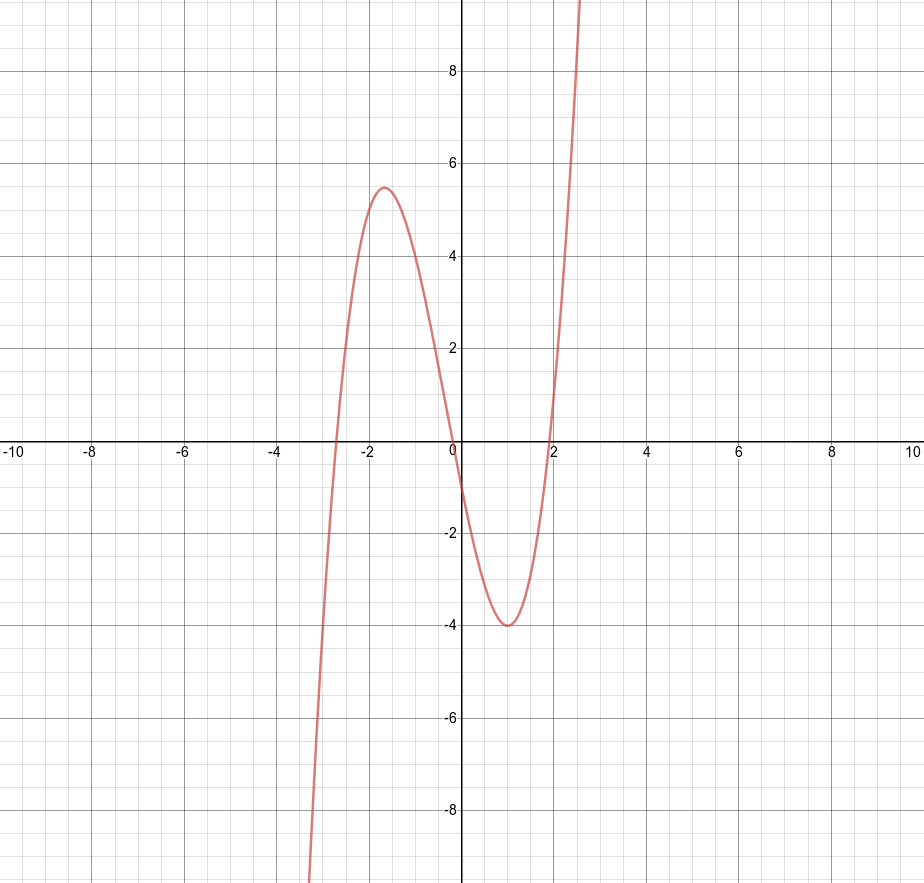
\includegraphics[scale=.3]{./diagrams/extrema1.png}
% \end{figure}

% Command             10pt    11pt    12pt
% \tiny               5       6       6
% \scriptsize         7       8       8
% \footnotesize       8       9       10
% \small              9       10      10.95
% \normalsize         10      10.95   12

\begin{document}

\begin{frame}
  \titlepage
\end{frame}

\begin{frame}
  \frametitle{Probability Distributions: Concepts}
Here are some definitions.
\begin{description}
\item[random variable] A random variable is a variable (typically
  represented by $X$) that has a single numerical value, determined by
  chance, for each outcome of a procedure.
\item[probability distribution] A probability distribution is a
  description that gives the probability for each value of the random
  variable. It is often expressed in the format of a table, formula,
  or graph.
\end{description}
\end{frame}

\begin{frame}
  \frametitle{Probability Distributions: Discrete and Continuous}
\begin{description}
\item[discrete random variable] A \alert{discrete} random variable has
  a collection of values that is finite or countable.
\item[continuous random variable] A \alert{continuous} random variable has
  infinitely many values, and the collection of values is not
  countable.
\item[countability] This is best explained by example: the integers
  are countable, but the real numbers are not.
\end{description}
\end{frame}

\begin{frame}
  \frametitle{Discrete Probability Distributions}
  If there are a finite number of outcomes $X=a_{k}$ for
  $k=1,\ldots,n$, we can list the values of $P(X=a_{k})$ in a table. 

\bigskip

\beispiel{Coin Toss}\label{ex:ootiteij} let $X=1$ for heads and $X=0$
for tails. Then 

\bigskip

\begin{tabular}{|l|l|}\hline
  Event & Probability \\ \hline
  $X=1$ or $H$ & 0.50 \\ \hline
  $X=0$ or $T$ & 0.50 \\ \hline
\end{tabular}

\bigskip

When all the probabilities are equal, we call the probability
distribution a \alert{uniform distribution}.
\end{frame}

\begin{frame}
  \frametitle{Non-Uniform Discrete Probability Distributions}
  Some distribution probability distributions are not uniform.

\bigskip

  \beispiel{Number of Male Children}\label{ex:shaisail} Consider the
  two-child family. If $X$ is the random variable corresponding to the
  number of boys in the family, then the probability distribution
  table looks as follows (assuming that the probability distribution
  for one child is uniform).
\end{frame}

\begin{frame}
  \frametitle{Discrete Probability Distribution Graphs I}
\begin{tabular}{|l|l|}\hline
  Event & Probability \\ \hline
  $X=2$ or two boys & 0.25 \\ \hline
  $X=1$ or one boy, one girl & 0.50 \\ \hline
  $X=0$ or two girls & 0.25 \\ \hline
\end{tabular}

\bigskip

\begin{figure}[h]
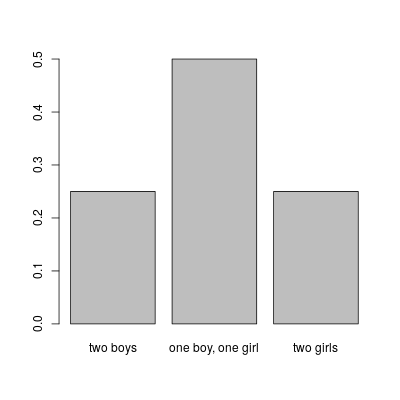
\includegraphics[scale=.45]{./diagrams/boys.png}
\end{figure}
\end{frame}

\begin{frame}
  \frametitle{Discrete Probability Distribution Graphs II}
  \beispiel{Immigrant Languages}\label{ex:ahchoiyu} Here is the
  probability distribution for a randomly selected ``Vancouverite''
  (Greater Vancouver) to speak a certain immigrant language at home.

\vspace{-.5in}

\begin{figure}[h]
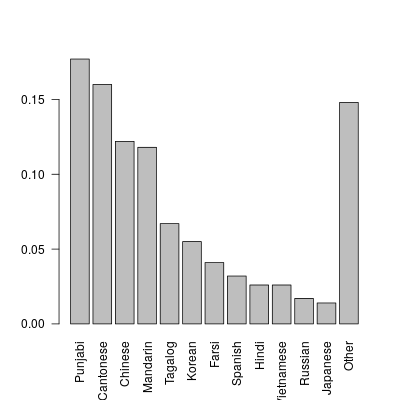
\includegraphics[scale=.5]{./diagrams/vanlang.png}
\end{figure}
\end{frame}

\begin{frame}
  \frametitle{Mean and Variance Formulas}
There is a sense in which a probability distribution together with its
associated random variable correspond to a population and the property
which the random variable picks out. In this spirit, let us define a
mean and a variance for a probability distribution.
\begin{equation}
  \label{eq:noohahfa}
  \mu=\sum{}X\cdot{}P(X)
\end{equation}
\begin{equation}
  \label{eq:axiengeb}
  \sigma^{2}=\sum(X-\mu)^{2}\cdot{}P(X)
\end{equation}
\begin{equation}
  \label{eq:teeneilu}
  \sigma^{2}=\sum(X^{2}\cdot{}P(X))-\mu^{2}
\end{equation}
\begin{equation}
  \label{eq:iifiekai}
  \sigma=\sqrt{\sum(X^{2}\cdot{}P(X))-\mu^{2}}
\end{equation}
\end{frame}

\begin{frame}
  \frametitle{Die Roll Example}
\beispiel{Fair Die Roll}\label{ex:reinooth} Think of rolling a fair die
many times. The probability distribution is uniform. The mean is
\begin{equation}
  \label{eq:isiamaih}
   \mu=\sum{}X\cdot{}P(X)=1\cdot{}\frac{1}{6}+2\cdot{}\frac{1}{6}+3\cdot{}\frac{1}{6}+4\cdot{}\frac{1}{6}+5\cdot{}\frac{1}{6}+6\cdot{}\frac{1}{6}=3.5\notag
\end{equation}
We also call this number the \alert{expectation} $EX$ of the random
variable $X$. Although you would never expect a die roll to result in
``3.5,'' you would expect the mean of many die rolls to be close to
this number. The expected number of boys for one birth is $EX=0.5$.
\end{frame}

\begin{frame}
  \frametitle{The Binomial Probability Distribution}
A \alert{binomial probability distribution} results from a procedure
that meets the following requirements.
\begin{enumerate}
\item The procedure has a fixed number of trials.
\item The trials must be independent.
\item The outcomes of a trial are binary, i.e.\ there are only two
  possible outcomes.
\item The probability of the two outcomes remains constant.
\end{enumerate}
The number of trials is usually labeled $n$, the two outcomes are
called \alert{success} and \alert{failure}, and their probabilities on
one trial are $p$ and $1-p$. The random variable keeps track of the
number of successes. If, for example, there are 10 trials, then
$P(X=4)$ is the probability of 4 successes out of 10. The number of
successes is often labeled $x$, and we are usually interested in
$P(X=x)$.
\end{frame}

\begin{frame}
  \frametitle{Calvin on the Binomial Distribution}
\begin{figure}[h]
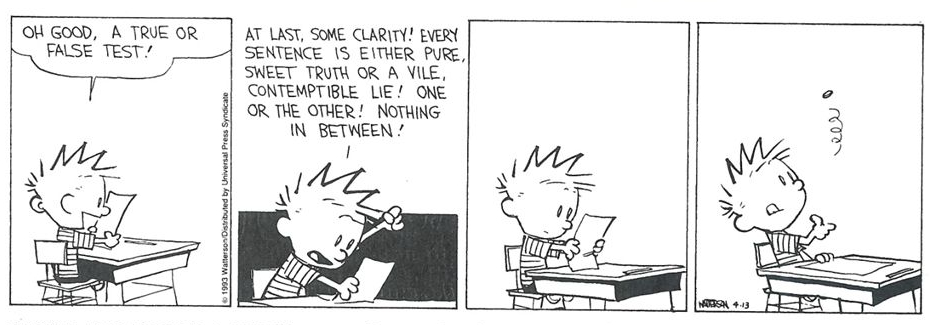
\includegraphics[scale=.43]{./diagrams/calvin_hobbes_binomial_edited.jpg}
\end{figure}
\end{frame}

\begin{frame}
  \frametitle{The Binomial Probability Formula}
If $n,p,x$ are as described on the previous slide, then
\begin{equation}
  \label{eq:pheehael}
  % P(X=x)={n\choose{}x}\cdot{}p^{x}\cdot(1-p)^{n-x}
  P(X=x)=\binom{n}{x}\cdot{}p^{x}\cdot(1-p)^{n-x}
\end{equation}
\end{frame}

\begin{frame}
  \frametitle{The Binomial Distribution and R}
Here are some R commands that help with the binomial distribution.

\bigskip

(1) Find the probability for 7 successes on 12 trials when the
probability of success is 40\% ($x=7,n=12,p=0.4$):
\begin{alltt}
  dbinom(7,12,0.4)\newline
  0.1009024
\end{alltt}
\end{frame}

\begin{frame}
  \frametitle{The Binomial Distribution and R}
(2) Do the same for $x=0,1,2,3,4,5$ and $n=5,p=0.40$:
\begin{alltt}
  dbinom(0:5,5,0.4)\newline
  0.07776 0.25920 0.34560 0.23040 0.07680 0.01024
\end{alltt}
(3) You can plot this distribution using (notice how skewed the
distribution is because of $p=0.40$):
\begin{alltt}
  x<-dbinom(0:5,5,0.4)\newline
  barplot(x)
\end{alltt}
\end{frame}

\begin{frame}
  \frametitle{The Binomial Distribution and R}
(4) Often, you want to add the probabilities for a range of $x$. For
example, what is the probability of having strictly fewer than 3
successes on 5 trials with $p=0.7$?
\begin{alltt}
  pbinom(2,5,0.4)\newline
  0.68256
\end{alltt}
(5) You can list these probabilities as follows:
\begin{alltt}
  pbinom(0:5,5,0.4)\newline
  0.07776 0.33696 0.68256 0.91296 0.98976 1.00000
\end{alltt}
\end{frame}

\begin{frame}
  \frametitle{The Binomial Distribution and R}
(6) You can simulate a binomial distribution using \texttt{rbinom}.
Conduct 100 experiments where you perform 12 trials with a success
probability $p=0.4$. Here are the results (number of successes $x$)
with a barplot:
\begin{alltt}
x<-rbinom(100,12,0.4)\newline
5 5 5 4 8 6 4 7 7 3 4 2 8 4 6 6 6 6 4 4 3 3 3 4 4 5 8 5 4 7 7 5 6 4 6 3 5
6 4 4 7 5 5 4 7 6 5 3 5 8 5 5 5 6 6 6 5 6 5 3 5 4 4 6 5 4 5 6 6 6 3 5 2 6
7 6 6 2 3 5 3 4 5 3 5 5 5 4 6 1 6 3 3 2 6 4 4 3 4 4\newline
barplot(table(x))
\end{alltt}
\end{frame}

\begin{frame}
  \frametitle{Exercises for the Binomial Distribution I}
  {\ubung} If you randomly guess on a multiple choice test with four
  possible answers, what is your probability of getting strictly more than 50\%
  of questions right when there are six questions?
\end{frame}

\begin{frame}
  \frametitle{Exercises for the Binomial Distribution II}
  {\ubung} The incidence of blue eyes in the population is 12\%. In a room
  with 20 randomly selected people, what is the probability of having
  three or more people with blue eyes? What is the probability of
  having strictly fewer than five people with blue eyes? 
  \begin{quote}
    Strictly speaking, the binomial probabilities are only approximate
    because the selection happens without replacement. If the
    population is large from which the sample is drawn, then you are
    allowed to ignore this.
  \end{quote}
\end{frame}

\begin{frame}
  \frametitle{Exercises for the Binomial Distribution III}
  {\ubung} Here is the distribution of blood types in Canada.

\bigskip

  \begin{tabular}{|l|r|r|r|r|}\hline
         & O     & A     & B     & AB    \\ \hline
Positive & 0.390 & 0.360 & 0.076 & 0.025 \\ \hline
Negative & 0.070 & 0.060 & 0.014 & 0.005 \\ \hline
  \end{tabular}

\bigskip

(a) What is the probability of being rhesus factor positive for
someone of blood type ``A''?

\medskip

(b) If you meet four randomly selected Canadians, what is the
probability that two of them are ``O'' positive?

\medskip

(c) In a room with twelve randomly selected Canadians, what is the
probability that there are strictly fewer than three people with
blood type ``B''?
\end{frame}

\begin{frame}
  \frametitle{Exercises for the Binomial Distribution IV}
  {\ubung} 80.5\% of US flights arrive on time. For twelve randomly
  selected flights, what is the probability that exactly ten of them
  are on time? What is the probability that between two and four of
  them are not on time?
\end{frame}

\begin{frame}
  \frametitle{Mean and Variance for the Binomial Distribution}
There are formulas for the mean and variance of the binomial
distribution. Especially the formula for the mean makes immediate
sense:
\begin{block}{Formulas}
  \begin{tabular}{llcr}
  mean& $\mu$&$=$&$np$ \\ 
  variance& $\sigma^{2}$&$=$&$npq$ \\
  standard deviation& $\sigma$&$=$&$\sqrt{npq}$
  \end{tabular}
\end{block}
It is a useful rule of thumb to remember that it is unlikely ($<5\%$)
that $x$ is outside of the interval from $\mu-2\sigma$ to
$\mu+2\sigma$.
\end{frame}

\begin{frame}
  \frametitle{Exercises for the Binomial Distribution V}
  {\ubung} What is the rule-of-thumb 95\% interval for the following
  binomial procedures:
  \begin{enumerate}
\item<1-> flipping a fair coin 15 times
\item<2-> answering 60 multiple choice questions with four possible
  answers for each question, where the probability of getting the right answer is 80\%
\item<3-> randomly answering 60 multiple choice questions with four
  possible answers for each question
\item<4-> The number of ``O'' positive blood types in a crowd of 100 Canadians.
  \end{enumerate}
\end{frame}

\begin{frame}
  \frametitle{Term Test A I}
  [6 points] What is the mean and what is the median population of a
  Canadian province/territory? These are the population numbers in
  1000s (census 2011):
\end{frame}

\begin{frame}
  \frametitle{Term Test A I}
  \begin{tabular}{|l|r|} \hline
Newfoundland and Labrador & 515   \\ \hline
Prince Edward Island      & 140   \\ \hline
Nova Scotia               & 922   \\ \hline
New Brunswick             & 751   \\ \hline
Quebec                    & 7903  \\ \hline
Ontario                   & 12852 \\ \hline
Manitoba                  & 1208  \\ \hline
Saskatchewan              & 1033  \\ \hline
Alberta                   & 3645  \\ \hline
British Columbia          & 4400  \\ \hline
Yukon                     & 34    \\ \hline
Northwest Territories     & 41    \\ \hline
Nunavut                   & 32    \\ \hline
\end{tabular}
\end{frame}

\begin{frame}
  \frametitle{Term Test A II}
  (2) [6 points] The father of modern sociology, {\'E}mile Durkheim,
  became famous for a study on suicide rates in Catholic and
  Protestant countries. Even though you would not be able to predict
  suicide for individuals or small groups, on a population level
  suicide rates are remarkably stable. Durkheim claimed that the
  suicide rate is significantly lower in Catholic populations than in
  Protestant populations. Let's assume the suicide rate for Catholics
  in a given country is 0.015\% and the suicide rate for Protestants
  is 0.04\%. If this country is predominantly Catholic (85\%), with
  15\% Protestants, then what is the probability that a person who has
  committed suicide is Catholic?
\end{frame}

\begin{frame}
  \frametitle{Term Test A III}
  (3) [6 points] You toss two coins. If there are no heads, you roll
  one die. If there are one or more heads, you roll two dice and add
  the two rolls. What is the probability that your result is six?
\end{frame}

\begin{frame}
  \frametitle{Term Test A IV}
  (4) [4 points] Events $X$ and $\urcorner{}Y$ are independent. Their
  joint probability is $0.18$. If $P(Y)=0.4$, then what is $P(X)$?
\end{frame}

\begin{frame}
  \frametitle{Term Test A V}
  (5) [6 points] Events $A$ and $B$ are disjoint. If $P(A)=0.2$ and
  $P(B)=0.4$, then what is $P(\urcorner{}A\cup\urcorner{}B)$? (Hint:
  contingency table.)
\end{frame}

\begin{frame}
  \frametitle{Term Test A VI}
  (6) [4 points] How many ways are there to draw samples of 5 persons
  from a population of 8 persons (order does not matter)?
\end{frame}

\begin{frame}
  \frametitle{Term Test A VII}
  (7) [6 points] Mother paints 60\% of her Easter eggs green and 40\%
  in other colours. Father paints 35\% of his Easter eggs green and
  65\% in other colours. There are one hundred eggs, 62 of which were
  painted by Father; the others by Mother. If you find a green egg,
  what is the probability that it was painted by Mother?
\end{frame}

\begin{frame}
  \frametitle{End of Lesson}
Next Lesson: Poisson and Normal Distribution
\end{frame}

\end{document}
